\chapter{Implementacija i korisničko sučelje}
		
		
		\section{Korištene tehnologije i alati}
		
			\textbf{\textit{dio 2. revizije}}
			
			 \textit{Detaljno navesti sve tehnologije i alate koji su primijenjeni pri izradi dokumentacije i aplikacije. Ukratko ih opisati, te navesti njihovo značenje i mjesto primjene. Za svaki navedeni alat i tehnologiju je potrebno \textbf{navesti internet poveznicu} gdje se mogu preuzeti ili više saznati o njima}.
			 
			 Komunikacija u timu realizirana je korištenjem aplikacije \textbf{\href{https://discord.com/}{Discord}}. 
			 Discord je društvena platforma na kojoj korisnici imaju mogućnost komuniciranja tekstualnim porukama, glasovnim
			 pozivima, videopozivima, medijima i datotekama u privatnim porukama ili kao dio zajednice koju nazivaju server. 
			 Za izradu UML dijagrama korišten je alat \textbf{\href{https://www.visual-paradigm.com/}{Visual Paradigm}}. Visual 
			 Paradigm je grafički alat koji omogućava jednostavno modeliranje mnogo različitih tipova UML dijagrama, poput 
			 dijagrama obrazaca uporabe, sekvencijskih dijagrama, dijagrama razreda, dijagrama stanja, dijagrama aktivnosti, 
			 dijagrama komponenata, ERD modela baze podataka i mnogih drugih. Za upravljanje izvornim kodom korišten je 
			 \textbf{\href{https://git-scm.com/}{Git}}. Git je open-source distribuirani sustav za upravljanje različitim 
			 verzijama datoteka. Udaljeni repozitorij projekta je dostupan na web platformi \textbf{\href{https://github.com/}{GitHub}}.
			 GitHub pruža usluge spremanja i upravljanja kodom. Koristi se Git-om kako bi omogućio upravljanje različitim 
			 verzijama datoteka. Također, GitHub omogućava dokumentiranje programske podrške pomoću wiki-ja.

			 Kao razvojno okruženje korišteni su \textbf{\href{https://code.visualstudio.com/}{Visual Studio Code}} 
			 i \textbf{\href{https://www.jetbrains.com/idea//}{Intellij IDEA}}. Visual Studio Code je uređivač teksta
			 razvijen u tvrtki Microsoft. Prvenstveno se koristi za razvoj računalnih sustava na operacijskom sustavu Windows. 
			 Korišten je za razvoj programske podrške na frontendu i razvoj dokumentacije. Intellij IDEA je integrirano razvojno 
			 okruženje (IDE) razvijeno u tvrtki JetBrains. Usmjereno je na razvoj Java aplikacija, no podržava niz drugih jezika i 
			 tehnologija. Korišten je za razvoj programske podrške na backendu.

			 Aplikacija je napisana koristeći radni okvir \textbf{\href{https://spring.io/projects/spring-boot}{Spring Boot}} i jezik 
			 \textbf{\href{https://www.java.com/en/}{Java}} za izradu \textit{backenda} te jezik \textbf{\href{https://www.javascript.com/}{JavaScript}} 
			 i njegovu biblioteku \textbf{\href{https://react.dev/}{React}} za izradu \textit{frontenda}. React je biblioteka 
			 u JavaScriptu za izgradnju korisničkih sučelja. Nastala je od strane Facebooka. Glavna karakteristika Reacta je komponentna 
			 arhitektura, što znači da se korisničko sučelje sastoji od više manjih, ponovno uporabljivih komponenata. Izrada 
			 složenijih aplikacija u Reactu obično zahtjeva korištenje dodatnih biblioteka za interakciju s API-jem. Radni okvir 
			 Spring Boot nudi gotova rješenja i funkcionalnosti koje ubrzavaju razvoj aplikacija. Ima automatsko upravljanje 
			 konfiguracijom i zavisnostima što olakšava i ubrzava posao programerima. Spring Boot pruža podršku za implementaciju 
			 sigurnosti u aplikacijama pomoću Spring Security modula. 

			 Baza podataka izvedena je u \textbf{\href{https://www.postgresql.org/}{PostgreSQL}}-u. PostgreSQL je open-source sustav za upravljanje relacijskim bazama
			 podataka kojim se proširuje funkcionalnost SQL-a. Dizajniran je da izdrži različita radna opterećenja, od 
			 pojedinačnih računala, pa sve do skladišta podataka ili web usluga s mnogo istodobnih korisnika. Baza podataka
			 se na poslužitelju u oblaku \textbf{\href{https://render.com/}{Render}}. Kao okruženje za upravljanje bazom
			 podataka korišten je open-source grafički alat \textbf{\href{https://www.pgadmin.org/}{pgAdmin}}.

		     Dokumentacija je pisana u jeziku \textbf{\href{https://www.latex-project.org/}{LaTeX}}. LaTeX je jezik za pisanje
			 strukturiranih tekstova profesionalne kvalitete. Za razliku od nekih programskih jezika za obradu teksta s grafičkim
			 sučeljem poput Microsoft Worda, dokumenti u LaTeX-u pisani su kao obični tekst s dodanom semantičkom strukturom. Time 
			 postiže usredotočenost na sadržaj, ujednačenost izgleda te brži i stabilniji rad.

			\eject 
		
	
		\section{Ispitivanje programskog rješenja}
			
			\textbf{\textit{dio 2. revizije}}\\
			
			 \textit{U ovom poglavlju je potrebno opisati provedbu ispitivanja implementiranih funkcionalnosti na razini komponenti i na razini cijelog sustava s prikazom odabranih ispitnih slučajeva. Studenti trebaju ispitati temeljnu funkcionalnost i rubne uvjete.}
	
			
			\subsection{Ispitivanje komponenti}
			\textit{Potrebno je provesti ispitivanje jedinica (engl. unit testing) nad razredima koji implementiraju temeljne funkcionalnosti. Razraditi \textbf{minimalno 6 ispitnih slučajeva} u kojima će se ispitati redovni slučajevi, rubni uvjeti te izazivanje pogreške (engl. exception throwing). Poželjno je stvoriti i ispitni slučaj koji koristi funkcionalnosti koje nisu implementirane. Potrebno je priložiti izvorni kôd svih ispitnih slučajeva te prikaz rezultata izvođenja ispita u razvojnom okruženju (prolaz/pad ispita). }
			
			
			
			\subsection{Ispitivanje sustava}
			
			 \textit{Potrebno je provesti i opisati ispitivanje sustava koristeći radni okvir Selenium\footnote{\url{https://www.seleniumhq.org/}}. Razraditi \textbf{minimalno 4 ispitna slučaja} u kojima će se ispitati redovni slučajevi, rubni uvjeti te poziv funkcionalnosti koja nije implementirana/izaziva pogrešku kako bi se vidjelo na koji način sustav reagira kada nešto nije u potpunosti ostvareno. Ispitni slučaj se treba sastojati od ulaza (npr. korisničko ime i lozinka), očekivanog izlaza ili rezultata, koraka ispitivanja i dobivenog izlaza ili rezultata.\\ }
			 
			 \textit{Izradu ispitnih slučajeva pomoću radnog okvira Selenium moguće je provesti pomoću jednog od sljedeća dva alata:}
			 \begin{itemize}
			 	\item \textit{dodatak za preglednik \textbf{Selenium IDE} - snimanje korisnikovih akcija radi automatskog ponavljanja ispita	}
			 	\item \textit{\textbf{Selenium WebDriver} - podrška za pisanje ispita u jezicima Java, C\#, PHP koristeći posebno programsko sučelje.}
			 \end{itemize}
		 	\textit{Detalji o korištenju alata Selenium bit će prikazani na posebnom predavanju tijekom semestra.}
			
			\eject 
		
		
		\section{Dijagram razmještaja}
			
			\textbf{\textit{dio 2. revizije}}
			
			 \textit{Potrebno je umetnuti \textbf{specifikacijski} dijagram razmještaja i opisati ga. Moguće je umjesto specifikacijskog dijagrama razmještaja umetnuti dijagram razmještaja instanci, pod uvjetom da taj dijagram bolje opisuje neki važniji dio sustava.}
			
			PLACEHOLDER
		
			\begin{figure}[H]
				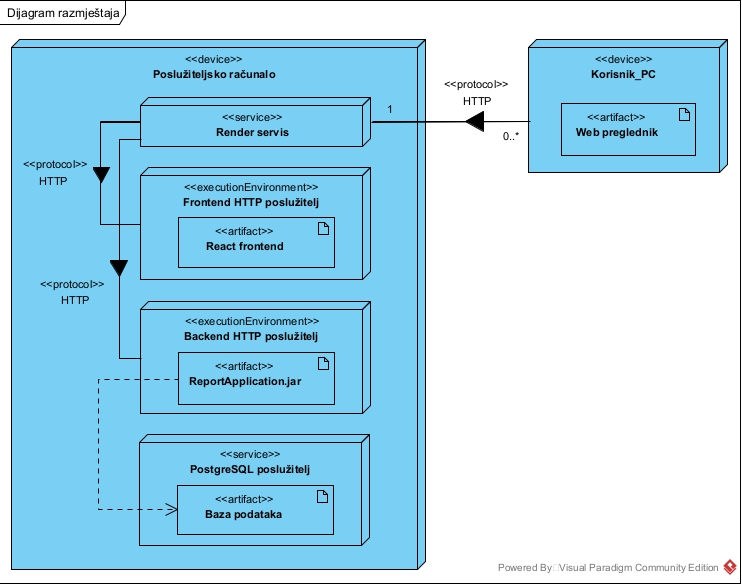
\includegraphics[scale=0.60]{slike/DR.jpg} %veličina slike u odnosu na originalnu datoteku i pozicija slike
				\centering
				\caption{Dijagram razmještaja}
				\label{fig:DijagramRazmjestaja}
			\end{figure}

			\eject 
		
		\section{Upute za puštanje u pogon}
		
			\textbf{\textit{dio 2. revizije}}\\
		
			 \textit{U ovom poglavlju potrebno je dati upute za puštanje u pogon (engl. deployment) ostvarene aplikacije. Na primjer, za web aplikacije, opisati postupak kojim se od izvornog kôda dolazi do potpuno postavljene baze podataka i poslužitelja koji odgovara na upite korisnika. Za mobilnu aplikaciju, postupak kojim se aplikacija izgradi, te postavi na neku od trgovina. Za stolnu (engl. desktop) aplikaciju, postupak kojim se aplikacija instalira na računalo. Ukoliko mobilne i stolne aplikacije komuniciraju s poslužiteljem i/ili bazom podataka, opisati i postupak njihovog postavljanja. Pri izradi uputa preporučuje se \textbf{naglasiti korake instalacije uporabom natuknica} te koristiti što je više moguće \textbf{slike ekrana} (engl. screenshots) kako bi upute bile jasne i jednostavne za slijediti.}
			
			
			 \textit{Dovršenu aplikaciju potrebno je pokrenuti na javno dostupnom poslužitelju. Studentima se preporuča korištenje neke od sljedećih besplatnih usluga: \href{https://aws.amazon.com/}{Amazon AWS}, \href{https://azure.microsoft.com/en-us/}{Microsoft Azure} ili \href{https://www.heroku.com/}{Heroku}. Mobilne aplikacije trebaju biti objavljene na F-Droid, Google Play ili Amazon App trgovini.}
			
			
			\eject 